\documentclass[8pt, landscape, fleqn]{scrartcl}
\setlength{\parindent}{0pt}
\usepackage[ngerman]{babel}
%\usepackage[applemac]{inputenc}
\usepackage[utf8]{inputenc}
\usepackage[dvips]{geometry}
\usepackage{latexsym}
\usepackage{multicol}
\usepackage{amsmath}
\usepackage{graphicx}
\usepackage{array}
\usepackage{booktabs}
\usepackage{amsmath}
\usepackage{mathtools}
\usepackage{ulem}
\usepackage{amsfonts}
\usepackage{dsfont}
\usepackage{charter} %%% Schreibart
%\renewcommand{\familydefault}{\sfdefault}



%%%%%%%%%%Paket für Chemische Formeln
\usepackage{chemformula} 
\usepackage[version=3]{mhchem}
%%%%%%%%%%%%%%%%% Farbe
\usepackage{color}

\pagestyle{plain}
\typearea{20}
\columnsep 30pt
\columnseprule .4pt
\setlength{\extrarowheight}{0.9em}

\renewcommand{\arraystretch}{0.8}

\makeatletter
\renewcommand{\section}{\@startsection{section}{1}{0mm}%
{-2\baselineskip}{0.8\baselineskip}%
{\hrule depth 0.2pt width\columnwidth\hrule depth1.5pt
width0.25\columnwidth\vspace*{1.2em}\Large\bfseries\rmfamily}}
\makeatother


\makeatletter
\renewcommand{\subsection}{\@startsection{subsection}{1}{0mm}%
{-2\baselineskip}{0.8\baselineskip}%
{\hrule depth 0.2pt width\columnwidth\hrule depth0.75pt
width0.25\columnwidth\vspace*{1.2em}\large\bfseries\rmfamily}}
\makeatother

\makeatletter
\renewcommand{\subsubsection}{\@startsection{subsubsection}{1}{0mm}%
{-2\baselineskip}{0.8\baselineskip}%
{\hrule depth 0.2pt width\columnwidth\vspace*{1.2em}\normalsize\bfseries\rmfamily}}
\makeatother

\newcommand{\Mx}[1]{\begin{bmatrix}#1\end{bmatrix}}
\begin{document}
\part*{\LARGE\textrm{Ökonomie $\hfill$ Xeno Meienberg}}
\begin{multicols*}{3}

\section{Einführung}

\subsection{Gegenstand der Ökonomie}

\begin{itemize}
    \item Mikroökonomie (2,3,5,6,7)
    \item Makroökonomie (8-11)
\end{itemize}

Die Mikroökonomie befasst sich mit wirtschaftlichen Entscheidungen der einzelnen Haushalte und Unternehmen:

\begin{itemize}
    \item Nachfrage (nach Gütern, Arbeit)
    \item Angebot (an Gütern, Arbeit)
    \item Marktgeschehen (Markformen, Marktpreise, Gleichgewichte)
\end{itemize}

Die Makroökonomie befasst sich mit gesamtwirtschaftlichen Zusammenhängen

\begin{itemize}
    \item Aussenwirtschaftstheorie und -politik 
    \item Geldtheorie und -politik 
    \item Arbeitsmarkttheorie und -politik 
\end{itemize}

Die Rolle der Ökonomie: 

\begin{itemize}
    \item Ökonomie ist eine Denkmethode
    \item ...ist eine Sozialwissenschaft
    \item ...keine eindeutige Wissenschaft
    \item beantwortet die Fragen:
    \item Warum Menschen könomische Entscheidungen treffen
    \item ...wie man aus knappen Ressourcen das Optimum herausholen kann
    \item ...dass Ziele möglichst gut erreicht werden 
    \item ...Ökonomisches Denken bedeutet die Warhnehmung von Zielkonflikten und das Auswählen von Alternativen
    \item ...Differenz zwischen Ertrag und Kosten maximiert wird
\end{itemize}

\subsection{Methodisches Vorgehen der Ökonomie}

\begin{enumerate}
    \item Feststelung eines Problems
    \item Analyse, Theorie, Modelle (Annahmen, Abstraktion, Empirische Tests)
    \item Politik (Handlungsempfehlungen)
\end{enumerate}

\subsection{Gesellschaftliche Bedeutung ökonomischer Analysen}

Grundidee: Knappe Ressourcen optimal einsetzen für grössten Nutzen (Wohlfahrt) Ressourcen sind:

\begin{itemize}
    \item Natürliche Ressourcen
    \item Human Ressources 
    \item Sachliche Ressourcen / Sachkapital
    \item Soziale Ressourcen / Spielregeln 
\end{itemize}

Eine der Hauptfragen der Ökonomie: Gegeben Potential (Ressoucenportfolio), was ist das Maxmimum an Wohlfahrt dass man erreichen kann? Die Kernfragen zu beantworten sind: 

\begin{enumerate}
    \item Was soll produziert werden?
    \item Wie sollen Güter und Dienstleistungen produziert werden?
    \item Wie und an wen sollen die produzierten Güter und Dienstleistungen verteilt werden? Wer konsumiert?
\end{enumerate}

\textbf{Transformationskuve}: Menge zweier Güter $X_1$ und $X_2$ (Outputs), die in einer Gesellschaft maximal bei gegebenen Ressourcen produziert werden können. \newline \newline
\textbf{Produktions-Effizienz}: Ein Güterbündel ist produktionseffizient, wenn es zu den minimal möglichen Kosten hergestellt wird oder wenn es zu gegebenen Kosten kein anderes Güterbündel gibt, für welches eines der beiden Güter grösser ist als möglich. Ein produktionseffizientes Güterbündel liegt auf der Transformationskuve. \newline \newline 
\textbf{Opportunitätskosten}: Ressultiert aus der Tatsache, dass Ressourcen knapp sind. Die Mehrproduktion eines Guts führt zu einer kleineren Menge eines anderen Guts. Die Minderproduktion werden Opportunitätskosten genannt. \newline \newline
\textbf{Indifferenzkurven}: Die Kurve stellt alle Outputkombinationen dar, zwischen denen die Gesellschaft (oder Individuum) indifferent ist. Je weiter die Indifferenzkurven vom Ursprung entfernt sind, umso höher ist der Nutzen (das Niveau) der jeweiligen Kurve \newline \newline
\textbf{Wohlfahrtsmaximum}: Ist der Punkt wo die Menge des Gutes 1 und 2 produziert werden müssen damit die Gesellschaft ihr Wohlfahrtsmaximum erreichen wird. (Muss auf der Transformationskuve sein) \newline \newline
\textbf{Allokations-Effizienz / Pareto-Optimal}: Eine Verteilung ist pareto-optimal, wenn keine Verteilung möglich ist, welche von mindestens einem Individuum bevorzugt wird, jedoch niemand anderes benachteiligt.  
\section{Haushalte und Nachfrage}

\subsection{Grundlegende Annahmen für Nachfrage- und Angebotsverhalten}

\textbf{Annahmen}
\begin{itemize}
    \item Raum: Keine Entfernungen vorhanden 
    \item Zeit: Zeit spielt keine Rolle 
    \item Güter: Güter sind homogen (Keine Qualitätsunterschiede zwischen Produkten)
    \item Personen: Es gibt keine Vorlieben oder Abneigungen (alle gleich)
    \item Informtationen: Es herrscht vollständige Informtationen (alle informiert über Markt für Entscheidungen)
\end{itemize}

\textbf{Ökonomische Entscheidungen} für private Haushalte 

\begin{itemize}
    \item Nachfrage von Gütern und Dienstleistungen
    \item Angebot von Ressourcen (Arbeit und Kapital)
    \item Konsum heute vs. morgen 
\end{itemize}

\subsection{Marktnachfrage nach Gütern und Dienstleistungen}

\textbf{Nachfrage}: $x^N$ ist eine Funktion des Preises $p$ eines Gutes. Üblicherweise sinkt die Nachfrage mit steigendem Preis. Grund hierfür sind empirisch oder durch Maximierung des Nutzens und Nebenbedingung der Budgetrestriktion 

\begin{center}
    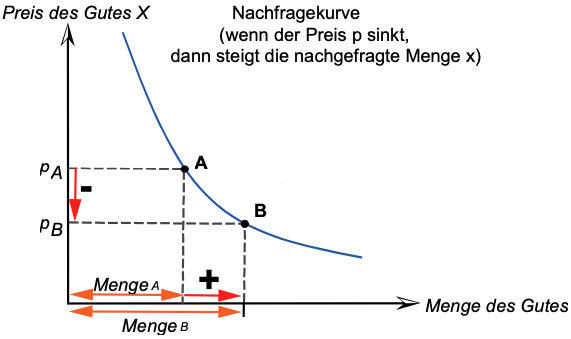
\includegraphics[width=7cm]{Typische_Nachfragefunktion.png}
\end{center}

\subsection{Ein Modell zu Konsumentscheidungen von Haushalten}

\subsubsection{Budgetrestriktion}

\textbf{Budgetrestriktion}: Summe der Ausgaben für zwei verschiedene Güter ($x_1p_1 + x_2p_2$) entsrpicht einem Budget $B$

\begin{align}
    B = x_1p_1 + x_2p_2 \\
    x_2 = \frac{B}{p_2} - x_1 \frac{p_1}{p_2}
\end{align}

Wie bereits erwähnt, ist der Nutzen eine lineare Kombination von preisen und Menge an Gütern, welche für eine Indifferenzkurve auf dem gleichen Niveau liegt die Gruppe oder Schar der Niveaulienen ergeben ein Nutzengebirge

\begin{equation}
    U = C x_1^a x_2^b
\end{equation}

mit $C$, $a$, $b$ Konstanten ($a,b =$ Bedeutung des Guts)

\subsubsection{Indifferenzkurven}

\textbf{Der Grenznutzen}: Ist die Ableitung einer Indifferenzkurve auf dem Niveau $U$ bezüglich $x_1$ und $x_2$ und ist immer positiv: 

\begin{equation}
    \frac{\partial U}{\partial x_1}, \frac{\partial U}{\partial x_2} > 0
\end{equation}

\textbf{Der Grenznutzen nimmt ab}. Der Nutzenzuwachs nimmt immer mehr ab mit zunehmenden Gütern einer Sorte (Es gitb eine Sättigung):

\begin{equation}
    \frac{\partial^2 U}{\partial x_1^2}, \frac{\partial^2 U}{\partial x_2^2} < 0
\end{equation}

Die Grenzrate der Substitution (GRS) misst die substituierbarkeit zweier Produkte und bestimmen die Form der Indifferenzkurve: 

\begin{equation}
   GRS =  \frac{GN_2}{GN_1} = \frac{dU/dx_2}{dU/dx_1}
\end{equation}

wobei perfekte Substitute bei $GRS = 1$ und perfekte Komplement bei $GRS = \pm \infty, 0$ 

\subsubsection{Der optimale Konsumpunkt}

\textbf{Der optimale Konsumpunkt}: Ist derjenige Punkt, wo sich Budgetrestriktion und Indifferenzkurve sich tangieren. Es ist dabei der maximale Nutzen bei gegebenem Budget. Die Steigung lautet hier $GRS$ bzw. $p_1/p_2$. Preisverhältnis = Grenzrate der Substitution/Grenznutzenverhältnis

\subsection{Von der optimalen Entscheidung zur individuellen Nachfragefunktion}

\begin{enumerate}
    \item Preis nimmt zu $\rightarrow$ Budgetrestriktion dreht sich 
    \item Es ergibt sich ein neues Nutzenniveau mit neuem Optimum
    \item Die nachgefragte Menge nimmt ab 
\end{enumerate}

Die Nachfragekurve zeigt die Zahlungsbereitschaft des Kosnumenten und kann auch als Funktion des Grenznutzens in Abhängigkeit von der Gütermenge interpretiert werden. Damit wird Nutzen und der marginale Nutzenzuwachs quantifizierbar und daher vergleichbar. 
Falls das Budget des Konsumenten sich ändert, oder seine Präferenzen sich änderen, kann verschiebt sich die Nachfragekurve nach oben oder nach unten. 

\begin{center}
    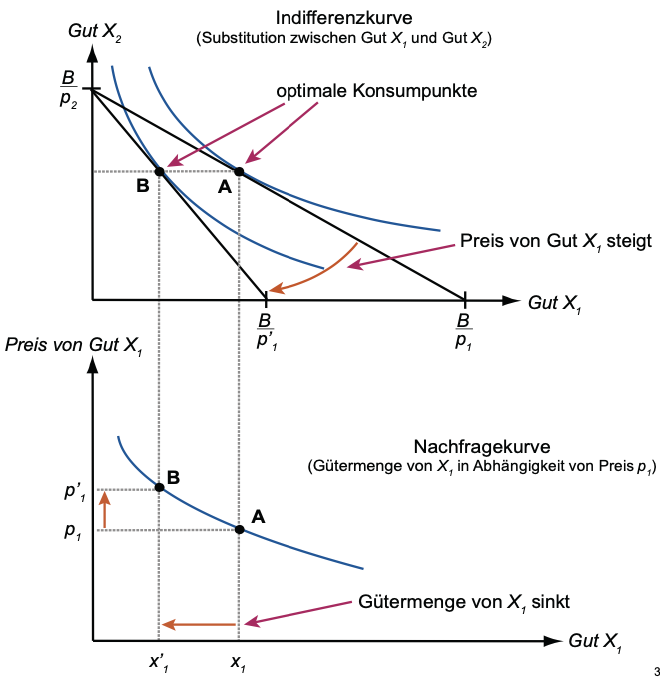
\includegraphics[width=7cm]{Nachfragefunktion.png}
\end{center}

\subsection{Preiselastizität der Nachfrage}

Die Preiselastizität der Nachfrage gibt an, um wie viel Prozent sich die nachgefragte Menge eines Gutes sich ändert als Folge einer einprozentigen Veränderung
des Preises dieses Gutes:

\begin{equation}
    \varepsilon_x N_p = \frac{\text{relative Mengenänderung}}{\text{relative Preisänderung}} = \frac{\frac{\Delta x^N}{x^N}}{\frac{\Delta p}{p}} = \frac{\Delta x^N}{\Delta p}\frac{p}{x^N}
\end{equation}

Im Grenzübergang $\Delta \rightarrow \partial$ beziehungsweise $\Delta p \rightarrow 0$:

\begin{equation}
    \varepsilon_x N_p = \frac{\partial x^N}{\partial p}\frac{p}{x^N}
\end{equation}

Die Preiselastizität hängt also von der Steigung der Nachfragekurve ($\frac{\partial x}{\partial p}$) und vom Preis/Mengenverhältnis ab. Entlang der Nachfragekurve variiert also die Elastizität. Da Nachfragekurven meist konvex sind, ist die die Preiselastizität negativ und nur der Betrag wird angegeben,
um das Ausmass zu repräsentieren. \newline \newline

Typen von Elastizität: 
    \begin{itemize}
        \item Vollkommen unelastisch ($\varepsilon = 0$): Preisänderung hat keinen Einfluss auf Nachfrage 
        \item Vollkommen elastisch ($\varepsilon = \pm \infty$): Preisänderung hat einen unendlichen grossen Einfluss auf Menge 
        \item Einheitselastisch ($\varepsilon = 1$): Preisänderung hat direkt gekoppelt mit Nachfrageverhalten 
        \item Elastisch ($\varepsilon > 1$): Die Nachfrage sinkt um mehr als ein Prozent wenn der Preis um 1 Prozent erhöht wird
        \item Unelastisch ($0<\varepsilon<1$): Die Nachfrage sinkt weniger als ein Prozent wenn der Preis um 1 Prozent erhöht wird
        \item Isoelastisch ($\varepsilon = const$): Die Nachfrage sinkt um einen konstanten Prozentsatz bei einer 1-prozentigen Erhöhung der Nachfrage
    \end{itemize}

Andere Arten der Elastizität: 

    \begin{enumerate}
        \item Einkommenselastizität der Nachfrage $\varepsilon_{x,Y}$: Veränderung der prozentualen Nachfragemenge eines Gutes $X$ aufgrund des veränderten Einkommens (Konsumbudget) $Y$. Diese ist meistens positiv (Konsum nimmt zu mit höherem Einkommen)
        \item Kreuzpreiselastizität $\eta_{x_1,p_2}$: Änderung der Nachfrage nach Produkt $X_1$ aufgrund er Preisänderung eines anderen Produkts $X_2$. Positive Kreuzpreiselastizitäten ergeben sich bei Substituten. Bei Komplementen ist die Kreuzpreiselastizität negativ 
    \end{enumerate}

\begin{align}
    \varepsilon_{x,Y} = \frac{\Delta x}{\Delta Y} \frac{Y}{x} \\
    \eta_{x_1,p_2} = \frac{\Delta x_1}{\Delta p_2}\frac{p_2}{x_1}
\end{align}

\section{Angebotsverhalten und Unternehmen}

\subsection{Güterangebot von Unternehmen bei volkommner Konkurrenz}

Zielvariable ist der Gewinn, der maximiert werden sollte. Randbedingungen: Güternachfrage und andere Unternehmen, die dasselbe Gut produzieren. Die Gewinnfunktion lautet (in Abhägnigkeit der Gütermenge $x$): 

\begin{equation}
    G(x) = E(x) - K(x) = px -K(x)=  \text{Erlös} - \text{Kosten}
\end{equation}

\begin{itemize}
    \item Notwendige Bedingung: $\frac{\partial G}{\partial x} = 0$ (Lok. Maximum / Minimum)
    \item Hinreichende Bedingung: $\frac{\partial^2 G}{\partial x^2} < 0$ (Negativ Gekrümmt)
\end{itemize}

Bei \textbf{Vollkommener Konkurrenz} gehen wir davon aus, dass einzelne Unternehmen keinen Einfluss auf den Preis haben. Wir bezeichnen den Preis $p$ als $\overline{p}$. Daraus folgt:

\begin{equation}
    \overline{p} = K' = \frac{\partial K}{\partial x} = E'
\end{equation}

\begin{itemize}
    \item $K'$: Grenzkosten: Gibt an, wieviel die zusätzlichen Kosten sind für jede weitere Produktion eines Gutes 
    \item $E'$: Grenzerlös: Zusätzlicher Erlös beim Verkauf jedes weiteren Gutes 
\end{itemize}

Die \textbf{Güterangebotsfunktion} ergibt sich, wenn man die Funktion $K'(x)$ explizit nach der Gütermenge auflöst:

\begin{equation}
    x^A = f(p),  \text{~mit } f'(p) > 0
\end{equation}

Die Grenzkostenkurve ist positiv steigend aufgrund der steigenden Kosten bei erhöhter Produktionsmenge. Die Kostenkurve ist in der Realität of durch eine S-förmige Kurve angenähert. Zuerst sinken die Grenzkosten (Kapazitätsauslastung steigt) und steigen nachher wieder an (Kapazitätsüberlastung) 

\begin{center}
    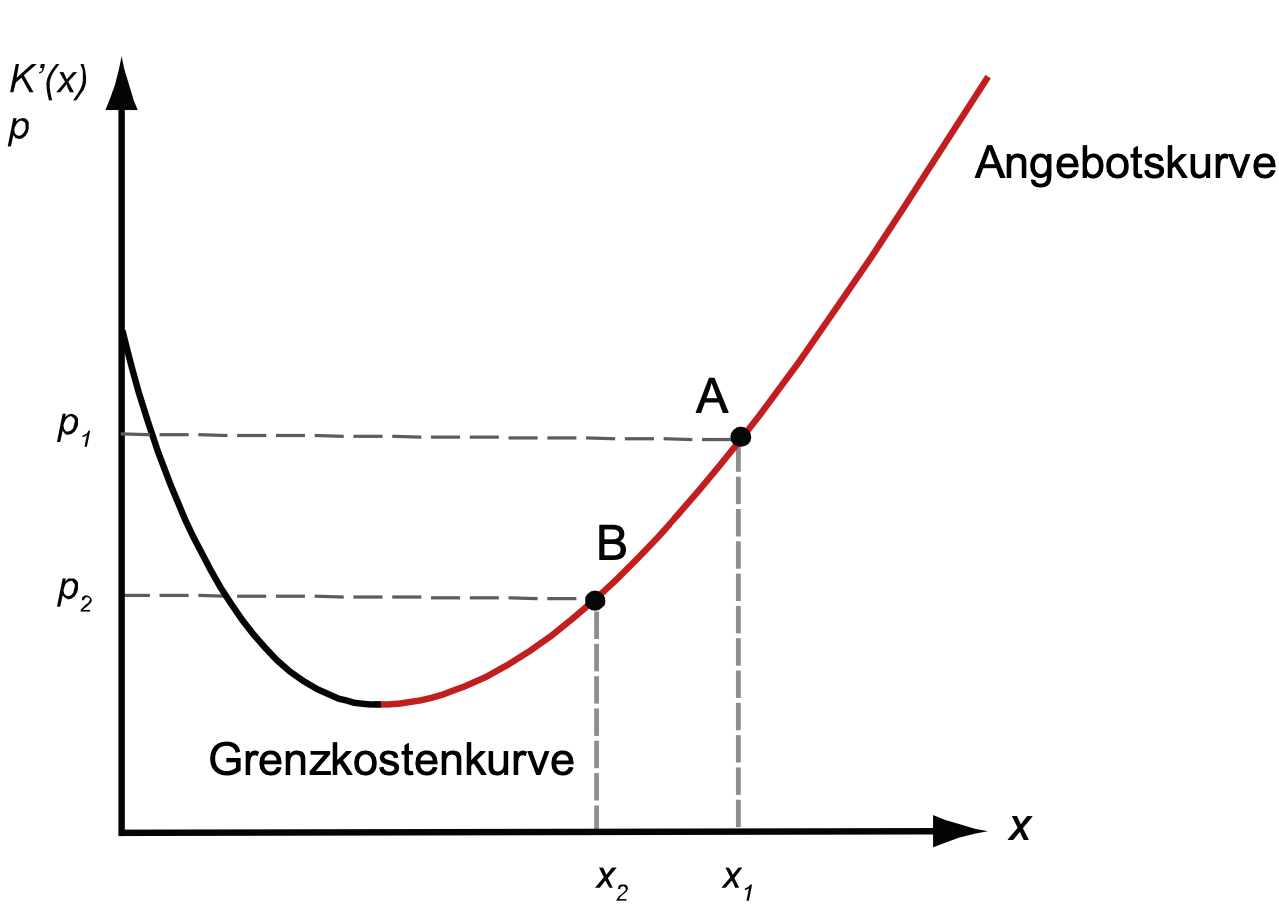
\includegraphics[width=6.5cm]{Gueterangebotsfunktion_Unternehmen.png}
\end{center}

\textbf{Kostenfunktion}: Abhängig von Fixkosten (von produzierten Menge unabhängig) und variable Kosten (von prod. Menge abhängig/steigen mit Produktionsmenge an). Die Grenzkosten sind unabhängig von den Fixkosten. Die Fixkosten bestimmen die Achsenverschiebung der Kostenfunktion. Die Kostenfunktion stellt den Zusammenhang zwischen Produktionsmenge und den jeweils minimalsten Kosten für $x$ dar.

\begin{equation}
    K(x) = K_{fix} + K_{var}(x)
\end{equation}

Die \textbf{Durchschnittkosten} $k$ beschreiben die Kosten pro Einheit:

\begin{equation}
    k(x) = K(x)/x
\end{equation}

Der \textbf{s-förmige Kostenverlauf}: Die Angebotskurve nimmt mit zunhemender Produktionsmenge nachdem die Grenzkosten erreicht worden sind zu. Bei Punkt $x_1$ sind die Kosten für jede weitere Produktion eines Gutes minimal. Die Steigung $\tan\alpha$ vom Ursprung aus ist dasselbe wie $k(x) = K(x)/x$ aus der Darstellung ersichtlich. Wenn man nun den Winkel in Abhängigkeit von $x$ plottet erhält man das Minimum der Durchschnittskostenkurve

\begin{center}
    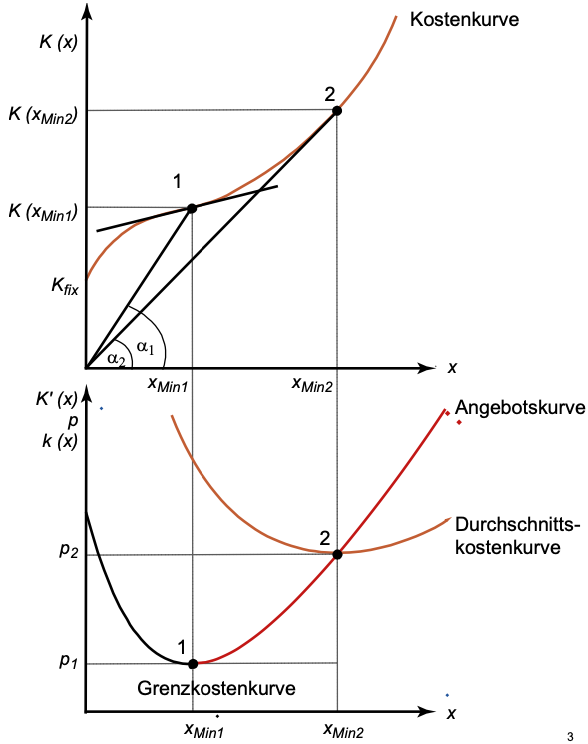
\includegraphics[width=8cm]{S-Foermiger-Kostenverlauf.png}
\end{center}

Die Produktionsfunktion bestimmt den s-förmigen Verlauf der Kostenfunktion. Mathematisch wird der Kostenverlauf folgendermassen definiert: 

\begin{equation}
    X = A a^\alpha k^\beta
\end{equation}

Wo $a$ die Arbeitsmenge und $k$ die Kapitalmenge repräsentieren. $A$, $\alpha$ und $\beta$ sind variable Parameter. 
Aufgrund der Form dieser Kurve (p. 5 / Kap. 3), kann man den Begriff der \textbf{Skalenerträge} definieren.Steigende Skalenerträge gehen mit fallenden Grenzkosten
bzw. langfristigen Durchschnittskosten einher. \newline \newline

\textbf{Langfristiges Betriebsminimum}: Ist der Ort, wo die Grenzkosten und die totalen Durchschnittskosten (TDK) gleich gross sind. Bei dieser Produktionsmenge sind die totalen Durchschnittskosten minimal und der Gewinn beträgt Null. \newline \newline
\textbf{Kurzfristiges Betriebsminimum}: Ist der Ort, wo die Angebotskurve die variablen Durchschnittskosten (VDK) schneiden (Firma möchte Fixkosten decken)

\begin{center}
    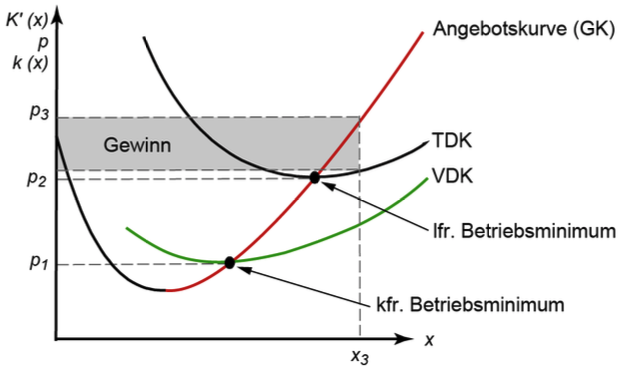
\includegraphics[width=7cm]{Betriebsminima.png}    
\end{center}



\subsection{Güterangebot eines Monopolisten}
\textbf{Monopol}: Ist eine Marktform, bei der es einen Anbieter und sehr viele, kleine Nachfrager gibt. Der Monopolist kann den Preis selbst bestimmen. Die zugehörige Menge wird bestimmt durch die Nachfragefunktion. Entstehungsgründe für ein Monopol:

\begin{itemize}
    \item Unternehmen hat Schlüsselressourcen, zu denen nur es Zugang hat (Diamanten z.B.)
    \item Wird vom Staat erschaffen, um einen Schlüsseldienst (Post) oder Urheberschutz gewährleistet wird (Bücher, Musik)
    \item Bei hohen Skalenerträgen, hohen Fixkosten und tiefen Grenzkosten. So lohnt es sich eher, dass nur eine Firma mit tieferen Durchschnittskosten besser produzieren kann als mehrere
\end{itemize}

Die Gewinnfunktion kann nun folgendermassen definiert werden und es gelten die gleichen Bedingungen wie bei vollständiger Konkurrenz, ausser dass nun der Preis $p(x)$ variabel ist:

\begin{align}
    G(x) = p(x) x - K(x) \\
    G'(x) = p'(x) x + p(x) 1 - K'(x) = 0\\
    G''(x) < 0 \Leftrightarrow K''(x) < p'(x)x + p(x)
\end{align}

Die Menge $x^*$, wo die notwendige und hinreichende Bedingung erfüllt ist, kann in die Nachfragefunktion eingesetzt werden ($p^* = p(x^*)$). Man nennt diesen Punkt \emph{Cournotpunkt}. Ändert sich die Nachfragekurve (Verschiebung, Drehung), so verändert sich die Lage des Cournotpunktes.



\subsection{Preiselastizität des Angebots}

Die \textbf{Preiselastizität des Angebots} gibt an, um wieviel Prozent sich die angebotene Menge eines Gutes verändert als Folge einer einprozentigen Veränderung des Preises dieses Gutes.

\begin{equation}
    \varepsilon_xA_p = \frac{\partial x^A}{\partial p}\frac{p}{x^A}
\end{equation}

Die Preiselastizität variiert in der Regel entlang der Kurve. Wir referenzieren $p$ und $x$ immer auf den Nominalwert (alten Wert)

\subsubsection{Verschiedene Elastizitätswerte}

Die Preiselastizität des Angebots ist meistens positiv aufgrund der Annahme, dass das Angebot mit steigendem Preis steigt. Falls:

\begin{itemize}
    \item $\epsilon_x A_p = 1$, dann geht die Angebotskurve durch den Ursprung
    \item $ \epsilon_x A_p > 1$, genau dann, wenn die Angebotskurve die Preisachse schneidet und ist undendlich bei $x^A = 0$ und konvergiert nach 1 für $x^A \rightarrow \infty$
\end{itemize}


\section{Kosten-Nutzen Analyse}

Grundlegendes Vorgehen: 

\begin{enumerate}
    \item Auflisten von Kosten und Nutzen über eine Laufzeit eines Projektes 
    \item Bestimmung des Nettonutzen pro Periode ($N_t-K_t$)
    \item Gewichtung der Nettonutzen nach zeitlichem Anfall (NPV)
    \item Auswahl: Handlungsalternative mit positiven NPV zu wählen oder andere Entscheidungskriterien
\end{enumerate}

\subsection{Gegenstand}
Grundidee: Systematische Gegenüberstellung von Kosten und Nutzen. Individuum wird eine Aktivität/Handlungsalternative x nur dann ausführen, wenn deren Kosten (costs) kleiner sind als deren Nutzen (benefits). Hierbei muss ebenfalls beachtet werden, dass es intagible 
Kosten gibt (nicht messbar) sowie mögliche Opportunitätskosten nicht berücksichtigt werden beim Assessment solcher Kosten. In der Volkswirtschaft wird dann diejenige Alternative berücksichtigt, welche der
Gesellschaft netto am Grössten Nutzen bringt. 

\begin{equation}
    \text{Max} \sum_{t=1}^T \delta^t(B_t - C_t),~ B_t = \sum_{i=1}^I B_{it}~\text{und}~ C_t = \sum_{i=1}^T C_{it}
\end{equation}

$B_i$ kann man interpretieren als die Zahlungsbereitschaft eines Individuums (max. bereit zu bezahlender Betrag), und $C_i$ für die Aktivität erforderlichen Aufwendungen.

\subsection{Bestimmung von Kosten und Nutzen}
Werden Güter auf (vollständigen) Märkten gehandelt, so entsprechen deren Preise der marginalen Zahlungsbereitschaft eines durchschnittlichen Individu- ums und determinieren die bereitgestellte (gehandelte) Gütermenge. Werden Güter nicht auf einem Markt gehandelt, sondern durch den Staat bereitgestellt, müssen Kosten und Nutzen der Bereitstellung anderweitig ermittelt werden. Während Kosten oft aufgrund von Kostenrechnungen bereits monetär erfasst werden, werden Nutzen (Opportunitätskosten) i.d.R. mit Hilfe der Zahlungsbereitschaft bewertet.
\subsubsection{Indirekte Methoden (Revealed Preference)}

\begin{itemize}
    \item Kompensationsmethode bei Schäden: Welcher Wert an Gütern muss eingesetzt werden, um Schäden zu ersetzen. Z.B. geringer Fischfang wegen Wasserverschmutzung. Reparaturkosten in Marktwerten ausdrücken. Anwendbarkeit nur bei reversiblen Schäden.
    \item Aufwandmethode/Reisekostenmethode: Die Kosten, die einem Individuum aus dem Besuch eines Ortes entstammen. Man fragt nach, wieviel eine Person aufgewandt hat um von seinem Herkunftsort an eine Destination zu gelangen. Alle Individuen können so zusammengefasst werden und die Daten sind vergleichbar 
    \item Hedonische Preise: Zahlungsbereitschaft für Güter mit ähnlichen Charakteristika (z.B. Immobilien an Ort X vs. Y). Wie ändert sich der Preis eines Hauses, wenn die Luftverschmutzung um 1\% zunimmt? Vorgehen: $Preis = f(Eigenschaften)$, erste Ableitung ist der hedonische Preis 
\end{itemize}

\subsubsection{Direkte Methoden (Stated Preference)}

\begin{itemize}
    \item Contingent Valuation: Hier werden Individuen mit einem Szenario konfrontiert und direkt über ihre Zahlungsbereitschaft (Willingness to Pay) befragt. Auf der anderen Seite werden Individuen gefragt, für wieviel Geld sie auf dasselbe Gut verzichten würden, der sogenannten Aktzeptantbereitschaft (Willingness to Accept). Oft gilt $WTP < WTA$
    \item Discrete Choice Experiment: Es werden Eigenschaften eines Guts definiert. Daraus lassen sich die Eigenschaften als Vektor definieren mit mehreren Dimensionen. Mehrere Alternativen an Gütern werden Individuen gezeigt und so kann statischtisch bestimmt werden, was die Zahlungsbereitschaft eines Guts ist.
\end{itemize}

\textbf{Zeitpräferenz}: Geld, dass man in der Zukunft erhält, und nicht jetzt, hat für ein Individuum weniger wert. Aus diesem Grund wir der sogenannte Diskontierungsfaktor $0 \leq \delta \leq 1$ definiert (siehe Gl. 21). \newline \newline

\textbf{Diskontrate vs. Marktzinssatz}: Die Diskontrate wird oft bestimmt via des Marktzinssatz $r$ bestimmt. Wir nehmen an, es gibt einen Zins auf den Betrag den man heute besitzt. Nach einem Jahr ist der Betrag $(1+r)$ wert. Also ist der aktuelle Diskontfaktor $\delta = 1/(1+r)$ .
Zusätzlich können andere, theoretische Überlegungen gemacht werden und die Diskontrate abhängig von der Gesellschaft modellieren: $\delta = z + ng$, wobei

\begin{itemize}
    \item $z$: Die pure Zeitpräferenz ist
    \item $n$: Der abnehmende Grenznutzen des Konsums, ausgedrückt durch die Einkommenselastizität des Konsums $n$
    \item $g$: Die Wachstumsrate des Pro-Kopf Konsums 
\end{itemize}



\subsection{Umgang mit Zeitkomponente}
\textbf{Barwertmethode und Net Present Value (NPV)}: 

\begin{equation}
    NPV = \sum_{t=0}^T \delta^t \left( N_t - K_t\right),~ N_0 = 0
\end{equation}

\textbf{Nutzen für zukünftige Generationen}: Hierbei ist zu beachten, dass es sich lohnt, zukünftige Einnahmen weniger abzudiskontieren. Der Nutzen ist langfristig angedacht und für zukünftige Generationen. Beispiel dafür sind Umwelthematiken. Hier kann man solche Projekte folgendermassen interpretieren: 

\begin{enumerate}
    \item Normale Diskontrate: Es handelt sich um ein Investitionsprojekt
    \item Tiefe Diskontrate: Weil sonst der Nutzen weggerechnet wird 
\end{enumerate}

\subsection{Unsicherheit}

\begin{itemize}
    \item Unsicherheit: Wir wissen nicht, mit welcher Wahrscheinlichkeit ein Ereignis auftritt
    \item Risiko: Es gibt Ereignisse oder Umweltzustände, über deren Eintreten wir nicht sicher sind aber wir kennen die Wahrscheinlichkeit (positives oder auch negatives Ereignis). Man kennt die objektive Wahrscheinlichkeit
    \item Ambiguität: Zwischenform von Unischerheit und Risiko. Der Entscheidungsträger entscheidet basierend auf subjektiver Wahrscheinlichkeit. 
    \item Erwartungswert: Werden für Risiken gemäss Statistik für Kosten wie auch Nutzen bestimmt $E(C) = \sum C_k p(C_k)$
    \item Risikoaversion: Viele Menschen würden anstatt auf den Erwartungswert immer eine sichere Alternative wählen. 
\end{itemize}


\subsection{Verteilungsproblematik}

\begin{itemize}
    \item Pareto-Effizienz: Grösstes Problem der Kosten-Nutzen-Analyse: Es sind keine Aussagen möglich, wie die Kosten und Nutzen innerhalb der Gesellschaft alloziert sind. Die Pareto-Effizienz ist ein Kriterium für die Einordnung der Verteilung
    \item Eine Güterverteilung gilt dann als effizient, wenn keine andere Güterverteilung möglich ist, welche mindestens ein Individuum besser, gleichzeitig aber kein anderes Individuum schlechter stellt 
    \item Gemäss K-N Analysen wird dann immer eine Massnahme empfohlen, wenn die Summe der Benefits die Summer der Kosten übersteigen, unabhängig von we die Kosten getragen werden. Diese Effizienz wird \emph{potentielle Pareto-Effizienz} genannt
\end{itemize}

Es ist wichtig anzumerken, dass die Kosten-Nutzen Analyse gute Resultate bringen kann, jedoch müssen die Parameter offengelegt sein.
\section{Analyse von Märkten}

\subsection{Aggregierte Angebots- und Nachfragekurven}

Die Aggregation findet horizontal statt. Je mehr Akteure,umso glatter wird die Angebotskurve/Nachfragekurve

\begin{center}
    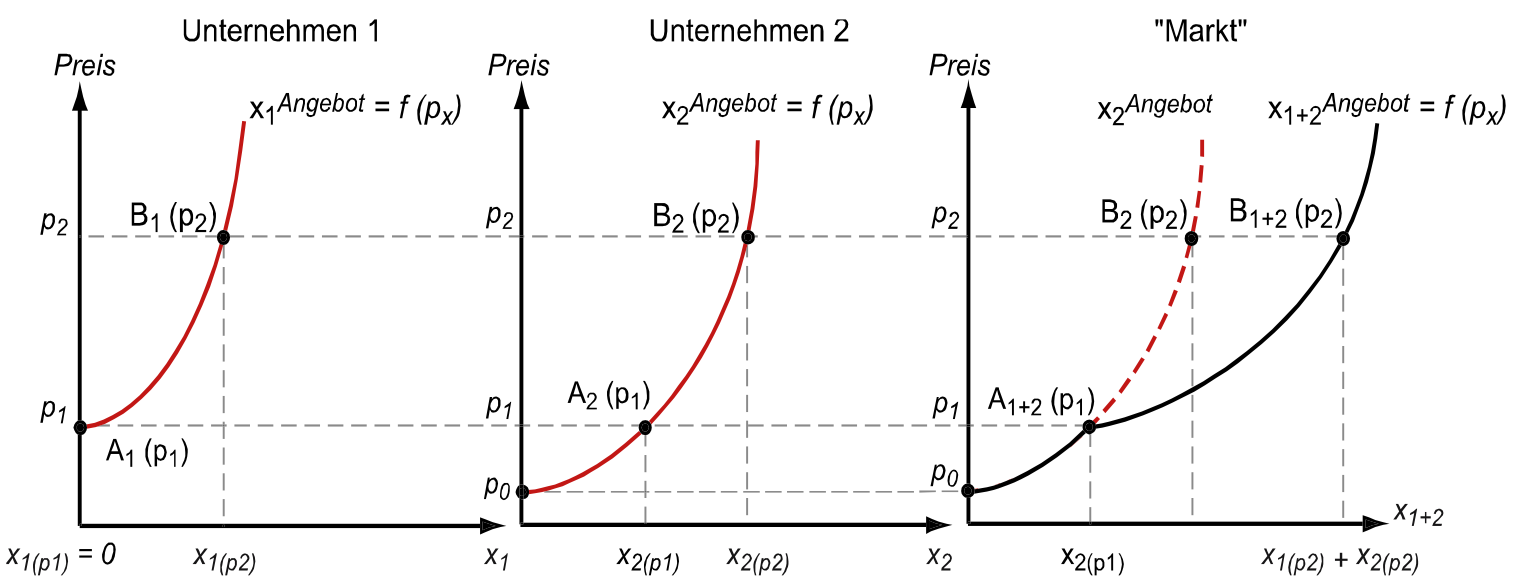
\includegraphics[width=8cm]{Angebotskurve_Aggregiert.png}
\end{center}

\subsection{Preisbildung auf Märkten}

\subsubsection{Preisbildung bei vollkommener Konkurrenz}

Annahme: Markt besteht aus vielen, kleinen Unternehmen und wird von vielen kleinen Haushalten in Anspruch genommen

\subsubsection{Preisbildung beim Monopol}

\subsubsection{Natürliches Monopol}

\subsection{Ökonomische Renten}

\subsubsection{Renten bei vollkommener Konkurrenz}

\subsubsection{Renten beim Monopol}

\subsubsection{Vergleich der Renten bei Konkurrenz und Monopol}

\subsection{Höchst- und Mindestpreise}

\subsubsection{Mindestpreise}

\subsubsection{Höchstpreise}

\subsection{Verbrauchssteuern}

\subsection{Subventionen}

\section{Öffentliche Güter und externe Effekte}

\section{Verhaltensökonomie}

\section{Leistungskraft und Wohlfahrt von Ökonomien}

\section{Arbeitslosigkeit}

\section{Aussenwirtschaft}

\section{Geld}


\end{multicols*}
\end{document}